\documentclass[tikz,border=10pt]{standalone}
\usepackage{amsmath,amssymb}
\usepackage{tikz}
\usetikzlibrary{arrows,automata,backgrounds,calendar,chains,decorations,decorations.pathreplacing,decorations.text,fit,matrix,mindmap,patterns,petri,plotmarks,positioning,shadows,shapes,shapes.callouts,shapes.geometric,shapes.misc,spy,trees,calc,intersections,tikzmark,arrows.meta}
\usepackage{xcolor}
\usepackage{pgfplots}
\pgfplotsset{compat=1.16}

% Common math macros from the book
\def\x{\mathbf{x}}
\def\y{\mathbf{y}}
\def\z{\mathbf{z}}
\def\A{\mathbf{A}}
\def\b{\mathbf{b}}
\def\c{\mathbf{c}}
\def\w{\mathbf{w}}
\def\v{\mathbf{v}}
\def\u{\mathbf{u}}
\def\e{\mathbf{e}}
\def\zero{\mathbf{0}}
\def\R{\mathbb{R}}
\def\N{\mathbb{N}}
\def\Z{\mathbb{Z}}
\def\Q{\mathbb{Q}}
\def\st{\text{s.t.}}
\def\vect#1{\mathbf{#1}}
\def\xLP{x^{\mathrm{LP}}}
\def\zLP{z^{\mathrm{LP}}}
\def\xIP{x^{\mathrm{IP}}}

% Common node styles from the book
\tikzset{
    main/.style={circle, draw, fill=gray!20, minimum size=1cm, font=\normalsize},
    dot/.style={circle,fill=blue,minimum size=3pt,inner sep=0pt, outer sep=-1pt},
    vertex/.style={circle,fill=black!25,minimum size=20pt,inner sep=0pt},
    edge/.style={draw,-,thick},
    directed edge/.style={draw,->,>=latex,thick},
}

% Additional macros for 3D/coordinate systems
\newcommand{\xhat}{\hat{\x}}
\newcommand{\yhat}{\hat{\y}}
\newcommand{\zhat}{\hat{\z}}
\newcommand{\ihat}{\hat{\imath}}
\newcommand{\jhat}{\hat{\jmath}}
\newcommand{\khat}{\hat{k}}

\begin{document}
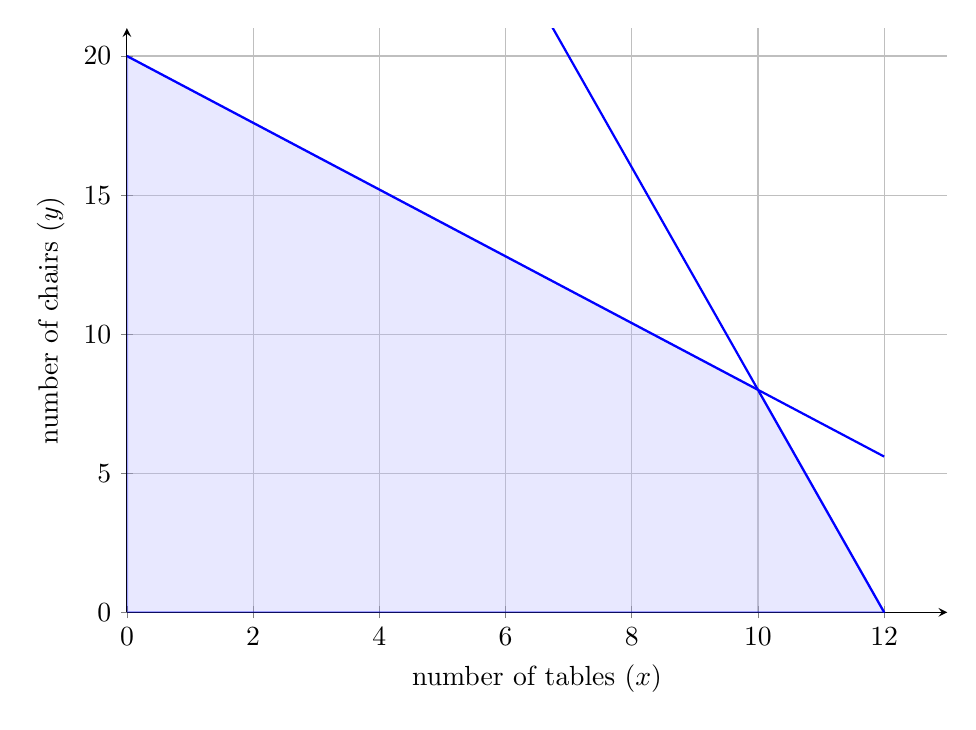
\begin{tikzpicture}
  \begin{axis}[
    xlabel={number of tables ($x$)},
    ylabel={number of chairs ($y$)},
    axis lines=left,
    xmin=0, xmax=13,
    ymin=0, ymax=21,
    xtick={0,2,4,6,8,10,12},
    ytick={0,5,10,15,20},
    width=12cm,
    height=9cm,
    grid=both,
    enlargelimits=false,
  ]

  % Feasible region (blue fill)
  \addplot[fill=blue!30, draw=blue, opacity = 0.3, thick] coordinates {
    (0,0)
    (0,20)
    (10,8)
    (12,0)
    (0,0)
  };

  % Constraint lines
  \addplot[domain=0:12, thick, blue] {48 - 4*x}; % 80x + 20y = 960
  \addplot[domain=0:12, thick, blue] {20 - 1.2*x}; % 12x + 10y = 200

  % Integer points in feasible region
%  \foreach \pt in {
%    (0,0), (0,20), (10,8), (12,0),
%    (1,18), (2,16), (3,14), (4,12), (5,10), (6,8), (7,6), (8,4), (9,2), (10,0)
%  } {
%    \addplot[only marks, mark=*, mark size=2pt, black] coordinates {\pt};
%  }
    % Objective function lines (example)


  \end{axis}
\end{tikzpicture}
\end{document}
